\documentclass{beamer}
\usetheme{Boadilla}
\usecolortheme{whale}
\graphicspath{{../../figures/}}

\usepackage{wrapfig}

\title[Thesis 1]
{First thesis presentation}

\subtitle{How far have I gone}

\author[V. BARBAZA]{Valentin BARBAZA}

\date[2023] % (optional)
{March 2023}

\logo{
\includegraphics[height=0.7cm]{logos/ist}}

\definecolor{istblue}{RGB}{0,102,153}
\setbeamercolor{titlelike}{bg=istblue}
\setbeamerfont{title}{series=\bfseries}

\begin{document}

\frame{\titlepage}

\begin{frame}
  \frametitle{Table of Contents}
  \tableofcontents
\end{frame}

\section{What I have done}

\begin{frame}{What I have done}
  Here are the things that I have done to this day.
  \begin{itemize}
    \item Implement Memristors in cadence
    \item Understand most of LSTMs
    \item Read and understand back-propagation
    \item Started writing thesis (Very beginning)
  \end{itemize}
\end{frame}

%\subsection{The Memristors}
\begin{frame}{Memristor implementation}
  Here are the resulting curves I obtained. The curves are the exact same ones as in the paper. Nevertheless, this type of memristor (changing by applying large voltage) probably isn't suitable for out system. It would require too long of a time to update the weights.
  \begin{figure}
    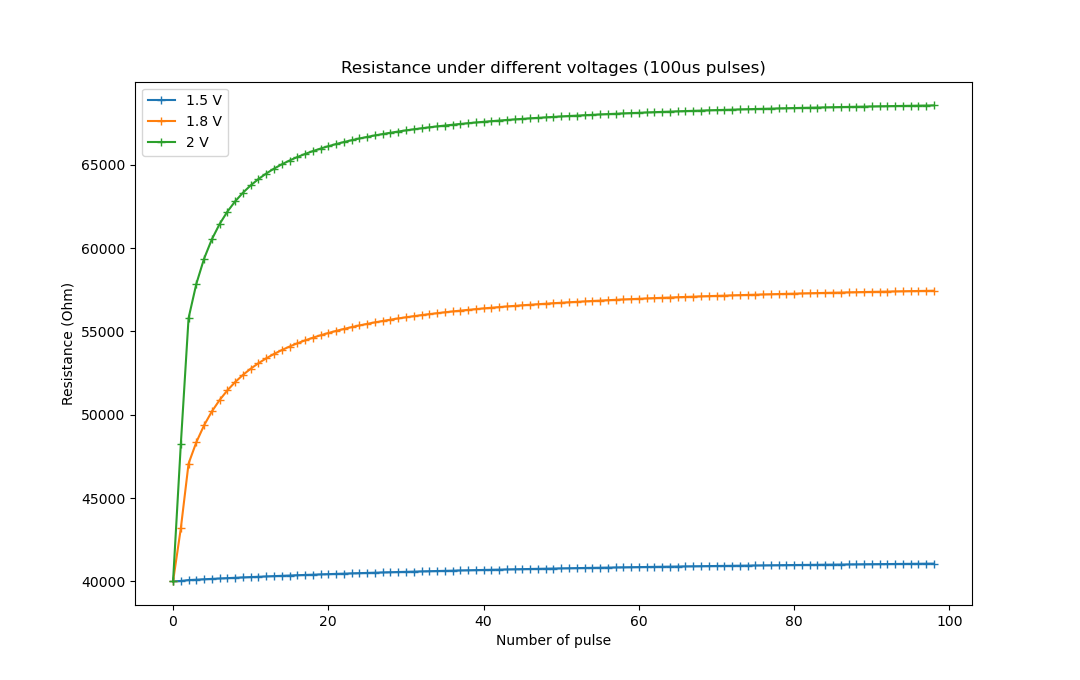
\includegraphics[height=0.5\textheight]{memristor/resistances-100us.png}
  \end{figure}
\end{frame}

\section{LSTM}
\begin{frame}{LSTM}
  \begin{figure}
    \centering
    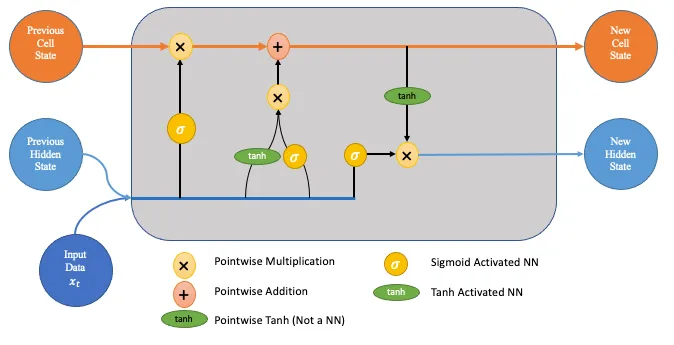
\includegraphics[width=\textwidth]{lstm/lstm.png}
  \end{figure}
\end{frame}
\begin{frame}{LSTM}
  \begin{figure}
    \centering
    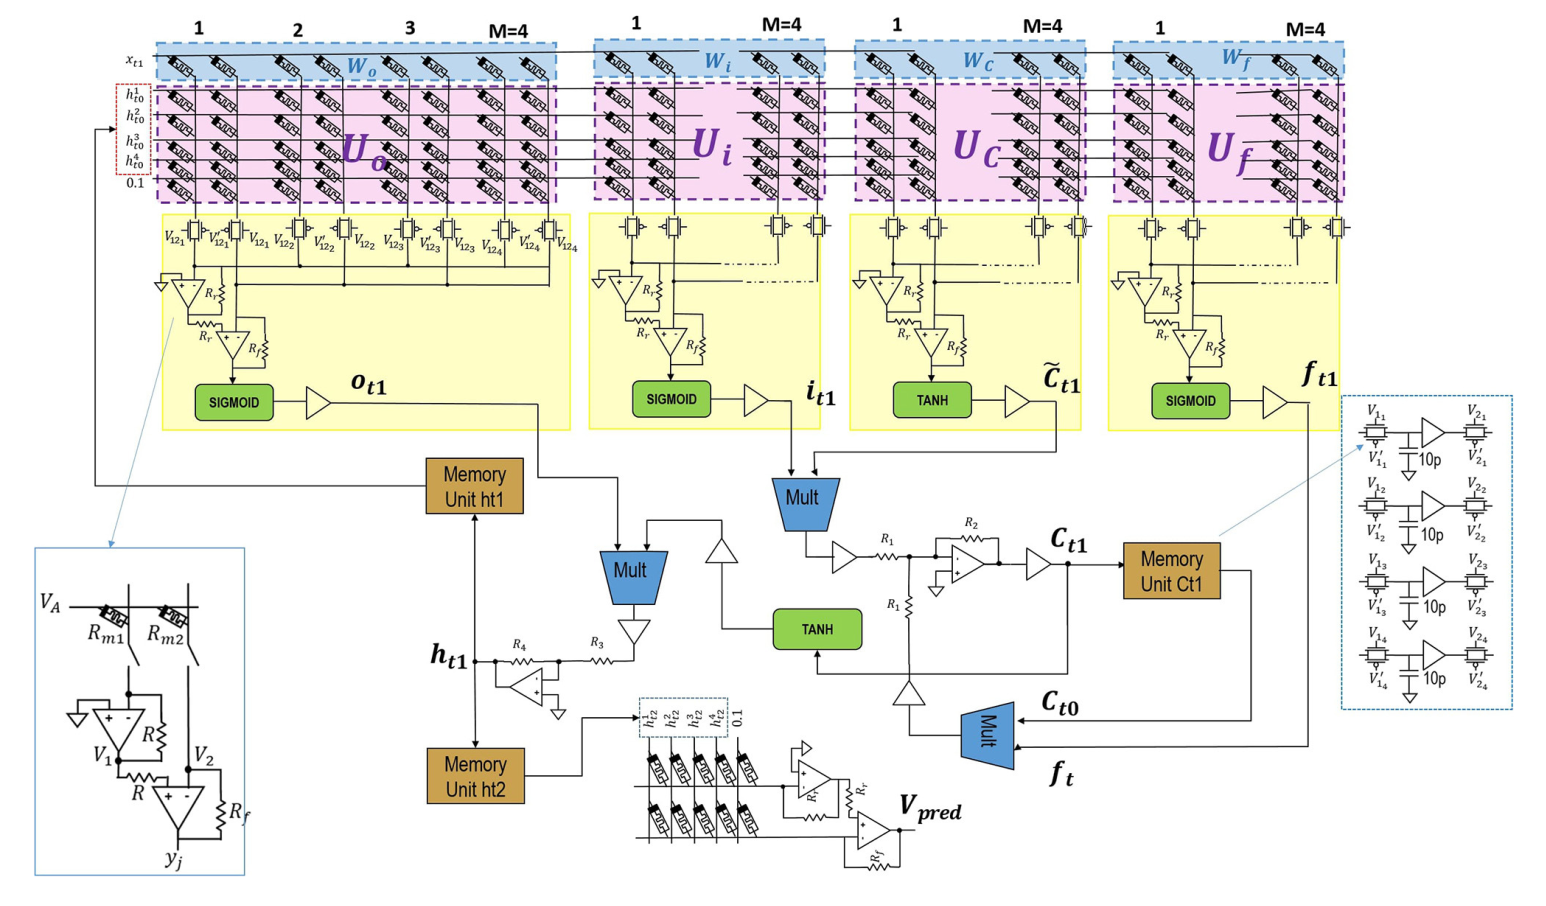
\includegraphics[width=0.9\textwidth]{lstm/analog-lstm.png}
  \end{figure}

\end{frame}

\section{What I can replicate}
\begin{frame}{What I can replicate}
  \begin{itemize}
    \item The circuit using resistances
    \item The circuit using pre-charged memristors
    \item Same for all LSTMs architectures
    \item Try to implement back-propagation (HARD)
    \item Compare power usage ?
  \end{itemize}
\end{frame}

%\begin{frame}{Back-propagation}
%   I think it would require a whole other system on the side, to calculate the new weights.
%\end{frame}

\section{Questions}
\begin{frame}{Questions}
  \begin{itemize}
    \item How to feed the inputs to the simulation ?
    \item How are the values encoded ?
  \end{itemize}
\end{frame}

\begin{frame}{Questions}
  For training :
  \begin{itemize}
    \item How long does it take to back-propagate ?
    \item Is the expected value, the value for next time step?
    \item Does that mean that the known values are for training ? Constant training in real time ?
  \end{itemize}
\end{frame}

\end{document}
